\documentclass[a4paper,10pt]{beamer}

\usepackage{préambule}
\usepackage{tcolorbox}
\usetikzlibrary{lindenmayersystems}

\tikzset{
  Koch curve/.style = {
    l-system={
      rule set={F -> F-F++F-F},
      axiom=F++F++F,
      step=1pt,
      angle=60,
      #1
    }
  }
}

\title{Flocon de Koch}
\date{}
\author{}

\begin{document}

\begin{frame}
	\begin{center}
		{\Large Flocon de Koch}

		\vspace{2em}

		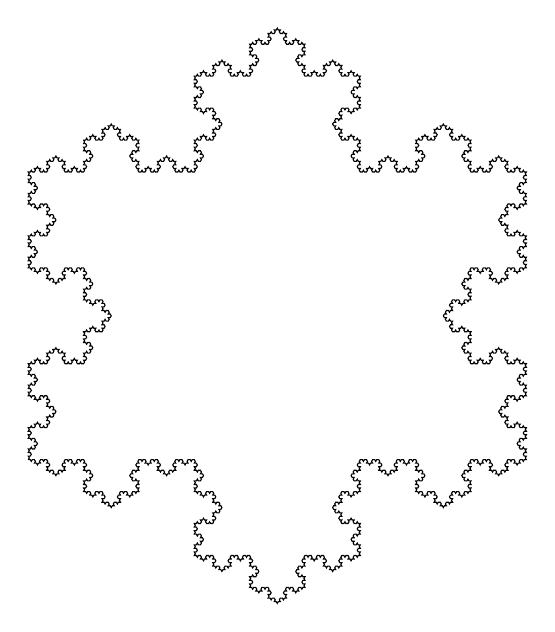
\begin{tikzpicture}
			\draw[Koch curve={order=5,step=180pt/3^(5)}] l-system;
		\end{tikzpicture}
	\end{center}
\end{frame}

\begin{frame}
	\hspace{-2em} 1. Premier dessin
	\begin{tcolorbox}
		\begin{itemize}
			\item[$∙$] Tracer un segment.
			\item[$∙$] Le découper en trois parties égales.
			\item[$∙$] Poser un triangle équilatéral sur le segment du milieu, et effacer sa base.
		\end{itemize}
	\end{tcolorbox}
	Si la longueur du segment de base est donnée, quelle est la longueur de la nouvelle figure ?

	\vspace{0.5em}

	\hspace{-2em} 2. On recommence la figure sur chaque petit segment ; puis sur chacun des segments de cette nouvelle figure ;

	et ainsi de suite ...
	\begin{itemize}
		\item[$∙$] Quelle est la longueur de la 4\textsuperscript{ème} figure ?
		\item[$∙$] Quelle est la longueur de la 10\textsuperscript{ème} figure ?
		\item[$∙$] Quelle est la longueur de la 103\textsuperscript{ème} figure ?
		\item[$∙$] Quelle est la longueur de la n\textsuperscript{ème} figure ?
	\end{itemize}
\end{frame}


\end{document}